\documentclass[tikz, border=4pt]{standalone}

\usepackage{amsmath,amssymb}
\usetikzlibrary{arrows.meta}
\usepackage{xcolor}

\definecolor{utnblue}{RGB}{0, 51, 102}
\definecolor{utnred}{RGB}{204, 0, 0}

\begin{document}
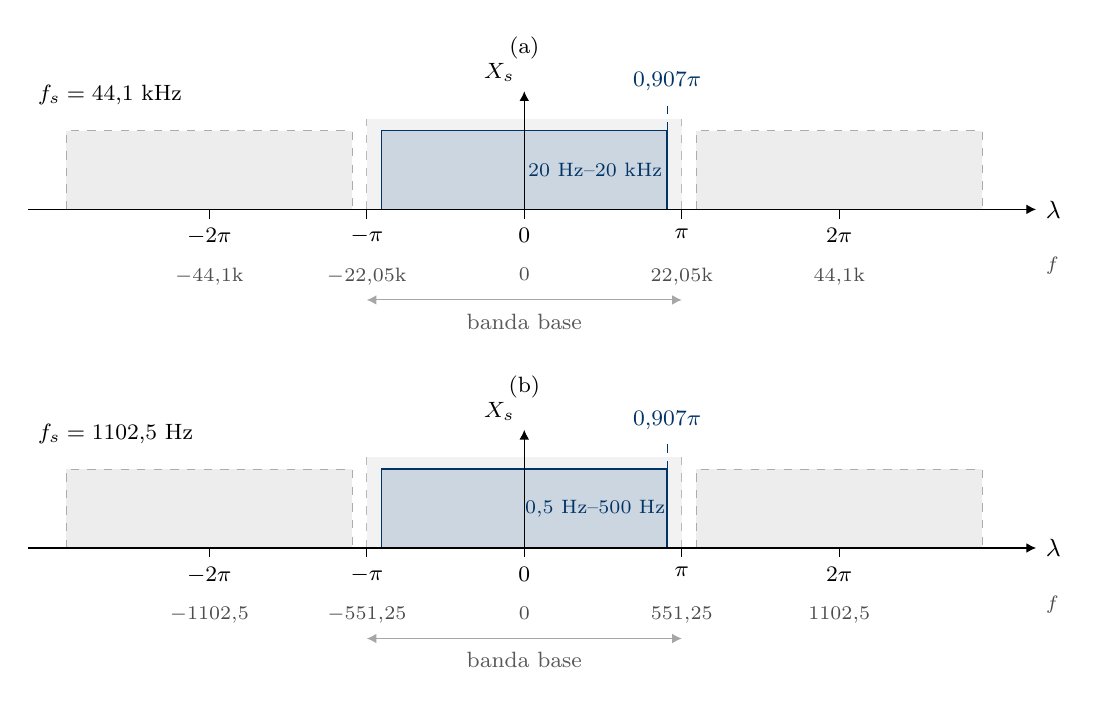
\begin{tikzpicture}[x=2.0cm, y=1cm, font=\small,
                    >={Latex[length=3.5pt,width=3.5pt]}]

    % ==========================================================
    % (a) audio, f_s = 44,1 kHz
    % ==========================================================
    \begin{scope}

        % banda base
        \fill[gray!10] (-1,0) rectangle (1,1.15);
        \draw[gray!55, thin, dashed] (-1,0) -- (-1,1.15);
        \draw[gray!55, thin, dashed] (1,0) -- (1,1.15);

        % imagenes
        \foreach \c in {-2,2} {
            \fill[gray!14] (\c-0.907,0) rectangle (\c+0.907,1);
            \draw[gray!65, thin, dashed] (\c-0.907,0) rectangle (\c+0.907,1);
        }

        % copia central
        \fill[utnblue!20] (-0.907,0) rectangle (0.907,1);
        \draw[utnblue, semithick] (-0.907,0) rectangle (0.907,1);
        \node[utnblue, font=\scriptsize] at (0.45,0.5) {$20$ Hz--$20$ kHz};

        % eje lambda, con la regla en Hz debajo
        \draw[->, thin] (-3.15,0) -- (3.25,0) node[right] {$\lambda$};
        \foreach \x/\l/\h in {-2/{$-2\pi$}/{$-44{,}1$k}, -1/{$-\pi$}/{$-22{,}05$k},
                              0/{$0$}/{$0$}, 1/{$\pi$}/{$22{,}05$k},
                              2/{$2\pi$}/{$44{,}1$k}} {
            \draw[thin] (\x,0) -- (\x,-0.12);
            \node[font=\footnotesize, anchor=north] at (\x,-0.12) {\l};
            \node[font=\scriptsize, gray!60!black, anchor=north] at (\x,-0.62) {\h};
        }
        \node[font=\scriptsize, gray!60!black, anchor=west] at (3.25,-0.72) {$f$};

        % eje de ordenadas
        \draw[->, thin] (0,0) -- (0,1.5) node[anchor=south east, font=\footnotesize] {$X_s$};

        % borde de la banda
        \draw[utnblue, thin, dashed] (0.907,1) -- (0.907,1.4);
        \node[utnblue, font=\footnotesize, anchor=south] at (0.907,1.38) {$0{,}907\pi$};

        % demarcacion de la banda base
        \draw[gray!70, thin, <->] (-1,-1.15) -- (1,-1.15);
        \node[gray!70!black, font=\footnotesize, anchor=north] at (0,-1.2) {banda base};

        \node[font=\footnotesize, anchor=west] at (-3.15,1.45) {$f_s = 44{,}1$ kHz};
        \node[font=\footnotesize] at (0,2.05) {(a)};

    \end{scope}

    % ==========================================================
    % (b) vibracion, f_s = 1102,5 Hz
    % ==========================================================
    \begin{scope}[yshift=-4.3cm]

        % banda base
        \fill[gray!10] (-1,0) rectangle (1,1.15);
        \draw[gray!55, thin, dashed] (-1,0) -- (-1,1.15);
        \draw[gray!55, thin, dashed] (1,0) -- (1,1.15);

        % imagenes
        \foreach \c in {-2,2} {
            \fill[gray!14] (\c-0.907,0) rectangle (\c+0.907,1);
            \draw[gray!65, thin, dashed] (\c-0.907,0) rectangle (\c+0.907,1);
        }

        % copia central
        \fill[utnblue!20] (-0.907,0) rectangle (0.907,1);
        \draw[utnblue, semithick] (-0.907,0) rectangle (0.907,1);
        \node[utnblue, font=\scriptsize] at (0.45,0.5) {$0{,}5$ Hz--$500$ Hz};

        % eje lambda, con la regla en Hz debajo
        \draw[->, thin] (-3.15,0) -- (3.25,0) node[right] {$\lambda$};
        \foreach \x/\l/\h in {-2/{$-2\pi$}/{$-1102{,}5$}, -1/{$-\pi$}/{$-551{,}25$},
                              0/{$0$}/{$0$}, 1/{$\pi$}/{$551{,}25$},
                              2/{$2\pi$}/{$1102{,}5$}} {
            \draw[thin] (\x,0) -- (\x,-0.12);
            \node[font=\footnotesize, anchor=north] at (\x,-0.12) {\l};
            \node[font=\scriptsize, gray!60!black, anchor=north] at (\x,-0.62) {\h};
        }
        \node[font=\scriptsize, gray!60!black, anchor=west] at (3.25,-0.72) {$f$};

        % eje de ordenadas
        \draw[->, thin] (0,0) -- (0,1.5) node[anchor=south east, font=\footnotesize] {$X_s$};

        % borde de la banda
        \draw[utnblue, thin, dashed] (0.907,1) -- (0.907,1.4);
        \node[utnblue, font=\footnotesize, anchor=south] at (0.907,1.38) {$0{,}907\pi$};

        % demarcacion de la banda base
        \draw[gray!70, thin, <->] (-1,-1.15) -- (1,-1.15);
        \node[gray!70!black, font=\footnotesize, anchor=north] at (0,-1.2) {banda base};

        \node[font=\footnotesize, anchor=west] at (-3.15,1.45) {$f_s = 1102{,}5$ Hz};
        \node[font=\footnotesize] at (0,2.05) {(b)};

    \end{scope}

\end{tikzpicture}
\end{document}
